\documentclass[12pt]{article}
\usepackage[utf8]{inputenc}
\usepackage{graphicx}
\usepackage{algorithm}
\usepackage{algpseudocode}

\title{Artificial Nose}
\author{Luca Belluardo e Andrea Stevanato}
\date{\today}

\begin{document}

\maketitle

\section{Introduction}
In this project a real-time application is developed to recognize smells from an
artificial nose. The sensor used for the application is an air quality gas sensor.

The rest of the documentation is structured in the following way: in section
2 the tasks are explained one at a time, in the section 3...

\section{The tasks}
In our application we have 7 periodic tasks (\ref{tdiagram}): graphic task, sensor task,
neural network task (made with Tensorflow), keyboard task and the store image
task.

The main function sets everything up for the tasks, except for the store
image task. The keyboard task is in charge to execute the store image task
when the \texttt{ENTER} key is pressed. If the store image task is already in
execution and the \texttt{ENTER} key is pressed this it's terminated.

Before start the store image task it's possible to write the name of the
directory in which the images will be saved; if no name it's writed the
images will be saved into \textit{image\_neural\_network} directory.

The sensor is readed by an Arduino M0 pro; the sampled data readed by arduino
are sent via the serial port to our application and readed by the sensor
task. All the tasks are terminated by the keyboard task when the user presses
the \texttt{ESC} key.

\begin{figure}[!t]
    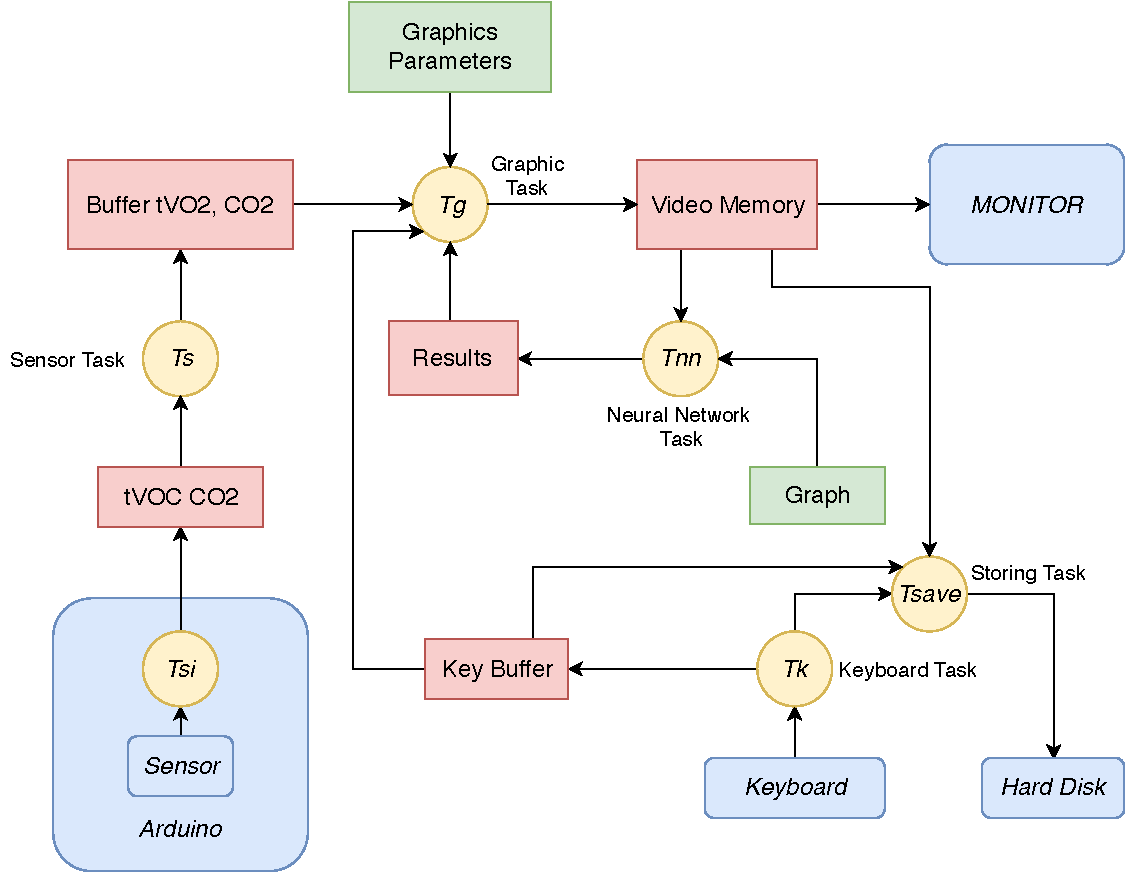
\includegraphics[width=\textwidth]{diagram.pdf}
    \caption{Task diagram}
    \label{tdiagram}
\end{figure}

\subsection{Main function}
In the main function(algorithm \ref{main}) all the tasks, except the store image task, are started
and the mutexes initialized. The mutexes are two, one for the data readed
from the sensor and the other for the results given by the neural network. 
The main also starts allegro and waits for the termination of the keyboard task.
Once the keyboard task terminates the main cancels all other task and wait for
their termination.

\begin{algorithm}[t]
\caption{Main}
\label{main}

\begin{algorithmic}
\State $T\gets$ \textit{tasks to be started}
\State \textit{Mutexes and allegro inizialization}
\For{$t \in T$}
    \State \textit{start} $t$
\EndFor

\Loop{ \textit{wait for termination of keyboard task}}
\EndLoop

\For{$t \in T$} 
    \State \textit{cancel and join} $t$
\EndFor

\end{algorithmic}
\end{algorithm}

\subsection{Graphic Task}

The graphic task is the one in charge to print the interface of our application.


\end{document}